\documentclass{article}
%% Packages:
    \usepackage{graphicx} % Used to insert images
    \usepackage{adjustbox} % Used to constrain images to a maximum size 
    \usepackage{xcolor} % Allow colors to be defined
    \usepackage{setspace}
    \usepackage{minted}
    \newminted[mysql1]{mysql}{
      mathescape,
      linenos=true, 
      texcl=true, 
      bgcolor=Background
      %gobble=2,
    }
    \newminted[python1]{python}{
      mathescape,
      linenos=true, 
      texcl=true, 
      bgcolor=Background
      %gobble=2,
    }

    %\usepackage{listings}
    \usepackage{float}
    \usepackage{enumerate} % Needed for markdown enumerations to work
    \usepackage{geometry} % Used to adjust the document margins
    \usepackage{amsmath} % Equations and \numberwithin command
    \usepackage{amssymb} % Equations
    \usepackage[T1]{fontenc}
    \usepackage{mdframed}
    \usepackage{newtxtext,newtxmath}
    \usepackage[utf8]{inputenc} % Allow utf-8 characters in the tex document
    \usepackage{fancyvrb} % verbatim replacement that allows latex
    \usepackage{grffile} % extends the file name processing of package graphics 
                         % to support a larger range 
    % The hyperref package gives us a pdf with properly built
    % internal navigation ('pdf bookmarks' for the table of contents,
    % internal cross-reference links, web links for URLs, etc.)
    \usepackage{tikz}
    \usepackage{pgfplots}
    \usepackage[]{ulem}
    \pgfplotsset{compat=newest}
    \usepackage{url}
    \usepackage{longtable} % longtable support required by pandoc >1.10
    \usepackage{booktabs}  % table support for pandoc > 1.12.2
    \usepackage{ulem} % ulem is needed to support strikethroughs (\sout)
    \usepackage{titlesec}
    %\titleformat{\section}{\normalfont\Large\bfseries}{Question {\thesection}: }{1em}{}
    \usepackage{hyperref}

    \renewcommand{\sectionautorefname}{\S}
    % Define a nice break command that doesn't care if a line doesn't already
    % exist.
    \def\br{\hspace*{\fill} \\* }
    % Math Jax compatability definitions
    \def\gt{>}
    \def\lt{<}
    % Document parameters

    \title{Analyzing the NYC Subway Dataset}
    \author{Yigal Weinstein}

    \sloppy 
    \usepackage[
      autocite=inline, 
      backend=biber,
      labeldate=true, 
      refsegment=section,
      uniquename=full,
      defernumbers=true,
      uniquelist=true]
    {biblatex}
    \addbibresource{udacity.bib}
    \PassOptionsToPackage{unicode}{hyperref}
    \PassOptionsToPackage{naturalnames}{hyperref}
    \hypersetup{pdfauthor={Yigal Weinstein},
      pdftitle={P2: Analyzing the NYC Subway Dataset},
      pdfsubject={data science, Udacity, MOOC},
      pdfkeywords={data science, statistics, probability, machine learning},
      pdfcreator={PdfLaTeX},
      %bookmarks={true},            %  A set of Acrobat bookmarks are written
      colorlinks={true},           %  Colors the text of links and anchors. 
      anchorcolor={black},         %  Color for anchor text.
      filecolor={cyan},            %  Color for URLs which open local files.
      menucolor={red},             %  Color for Acrobat menu items.
      runcolor={blue},              %  Color for run links (launch annotations).        
      linkcolor={red!50!black},
      citecolor={blue!50!black},
      urlcolor={blue!80!black},
      breaklinks=true,  % so long urls are correctly broken across lines
    }           

    \definecolor{Background}{rgb}{0.95,0.95,0.92}
    %\geometry{verbose,tmargin=1in,bmargin=1in,lmargin=1in,rmargin=1in}

\makeatletter

\def\@seccntformat#1{%
  \expandafter\ifx\csname c@#1\endcsname\c@section\else
  \csname the#1\endcsname\quad
  \fi}
  \newcommand{\ssection}[1]{
\phantomsection
\section*{#1}
\addcontentsline{toc}{section}{\protect\numberline{}#1}}

\newcounter{questionCtr}
\newenvironment{question}{%      define a custom environment
   \bigskip\noindent%         create a vertical offset to previous material
   \refstepcounter{questionCtr}% increment the environment's counter
   \textsc{Question \thequestionCtr}% or \textbf, \textit, ...
   \newline%
   }{\par\bigskip}  %          create a vertical offset to following material
\numberwithin{questionCtr}{section}

\newcounter{problemCtr}

\newenvironment{problem}{%      define a custom environment
   \bigskip\noindent%         create a vertical offset to previous material
   \refstepcounter{problemCtr}% increment the environment's counter
   \textsc{Problem \theproblemCtr}% or \textbf, \textit, ...
   \newline%
   }{\par\bigskip}  %          create a vertical offset to following material
\numberwithin{problemCtr}{section}

\@addtoreset{section}{part}

\makeatother

\begin{document}
\maketitle
\section*{Introduction}
This project attempts to follow the outline provided in \cite{Udacity-P2-DS}
and the project rubrick set forth in \cite{Udacity-P2-rubrick}.  It is divided
into two parts.  The first part, below, are answers to the short questions in
\cite{Udacity-P2-DS} while the second part contains the code and and notes
regarding problem set 2,3, and 4 of the Intro to Data Science course
\cite{Udacity-data-science-course}.
\part{Analyzing the NYC Subway Dataset}
\section{Statistical Test}
\label{sec:statistical_test_one}
\begin{question}
  Which statistical test did you use to analyze the NYC subway data? Did you use
  a one-tail or a two-tail P value? What is the null hypothesis? What is your
  p-critical value?
\end{question}

\begin{question}
  Why is this statistical test applicable to the dataset? In particular,
  consider the assumptions that the test is making about the distribution of
  ridership in the two samples.
\end{question}

\begin{question}
  What results did you get from this statistical test? These should include the
  following numerical values: p-values, as well as the means for each of the two
  samples under test.
\end{question}

\begin{question}
  What is the significance and interpretation of these results?
\end{question}

\section{Linear Regression}

\begin{question}
  What approach did you use to compute the coefficients theta and produce
  prediction for \verb|ENTRIESn_hourly| in your regression model:
  \begin{itemize}
    \item OLS using Statsmodels or Scikit Learn
    \item Gradient descent using Scikit Learn
    \item Or something different?
  \end{itemize}
\end{question}

\begin{question}
  What features (input variables) did you use in your model? Did you use any
  dummy variables as part of your features?
\end{question}

\begin{question}
  Why did you select these features in your model? We are looking for specific
  reasons that lead you to believe that the selected features will contribute to
  the predictive power of your model.
  \begin{itemize}
    \item Your reasons might be based on intuition. For example, response for
      fog might be: “I decided to use fog because I thought that when it is very
      foggy outside people might decide to use the subway more often.”
    \item Your reasons might also be based on data exploration and
      experimentation, for example: “I used feature X because as soon as I
      included it in my model, it drastically improved my R2 value.”
  \end{itemize}
\end{question}

\begin{question}
  What are the parameters (also known as ``coefficients'' or ``weights'') of the
  non-dummy features in your linear regression model?
\end{question}

\begin{question}
  What is your model’s $R^2$ (coefficients of determination) value?
\end{question}

\begin{question}
  What does this $R^2$ value mean for the goodness of fit for your regression
  model? Do you think this linear model to predict ridership is appropriate for
  this dataset, given this $R^2$  value?
\end{question}

\section{Visualization}
Please include two visualizations that show the relationships between two or
more variables in the NYC subway data.
Remember to add appropriate titles and axes labels to your plots. Also, please
add a short description below each figure commenting on the key insights
depicted in the figure.

One visualization should contain two histograms: one of  \verb|ENTRIESn_hourly| for
rainy days and one of \verb|ENTRIESn_hourly| for non-rainy days.
\begin{question}
  One visualization should contain two histograms: one of  \verb|ENTRIESn_hourly| for
  rainy days and one of \verb|ENTRIESn_hourly| for non-rainy days.
\begin{itemize}
  \item One visualization should contain two histograms: one of  \verb|ENTRIESn_hourly|
    for rainy days and one of \verb|ENTRIESn_hourly| for non-rainy days.
  \item If you decide to use to two separate plots for the two histograms,
    please ensure that the x-axis limits for both of the plots are identical. It
    is much easier to compare the two in that case.
  \item For the histograms, you should have intervals representing the volume of
    ridership (value of \verb|ENTRIESn_hourly|) on the x-axis and the frequency of
    occurrence on the y-axis. For example, each interval (along the x-axis), the
    height of the bar for this interval will represent the number of records
    (rows in our data) that have \verb|ENTRIESn_hourly| that falls in this interval.
  \item Remember to increase the number of bins in the histogram (by having
    larger number of bars). The default bin width is not sufficient to capture
    the variability in the two samples.
\end{itemize}
\end{question}

\begin{question}
  One visualization can be more freeform. You should feel free to implement
  something that we discussed in class (e.g., scatter plots, line plots) or
  attempt to implement something more advanced if you'd like. Some suggestions
  are:
  \begin{itemize}
    \item Ridership by time-of-day
    \item Ridership by day-of-week
  \end{itemize}
\end{question}

\section{Conclusion}
Please address the following questions in detail. Your answers should be 1-2
paragraphs long.
\begin{question}
 From your analysis and interpretation of the data, do more people ride
 the NYC subway when it is raining or when it is not raining?
\end{question}

\begin{question}
  What analyses lead you to this conclusion? You should use results from both
  your statistical tests and your linear regression to support your analysis.
\end{question}

\section{Reflection}
Please address the following questions in detail. Your answers should be 1-2
paragraphs long.

\begin{question}
Please discuss potential shortcomings of the methods of your analysis,
including:  
\begin{itemize}
  \item Dataset
  \item Analysis, such as the linear regression model or statistical test.
\end{itemize}
\end{question}

\begin{question}
  (Optional) Do you have any other insight about the dataset that you would like
  to share with us?
\end{question}
%\printbibliography[keyword=statistics , title={Statistics references}]
%\printbibliography[keyword=Matplotlib , title={Matplotlib references}]
%\printbibliography[keyword=SciPy , title={SciPy references}]
%\printbibliography[keyword=PANDAS , title={PANDAS references}]
\part{Code and Notes to Problem Sets 2,3 and 4}
\setcounter{section}{1}
What follows are my solutions to problem sets 2,3, and 4 of
\cite{Udacity-data-science-course}.
\section{Problem Set 2: Wrangling Subway Data}
%\ssection{Problem Set 2: Wrangling Subway Data}

% apparently the problems appear to have come from 
% http://usa-da.blogspot.com/2014/06/data-wrangling-project-2-wrangle-nyc.html
\begin{problem}
Number of Rainy Days
\end{problem}
The SQL query I used was,

\begin{mysql1}
SELECT COUNT(rain) FROM weather_data WHERE rain > 0.0
\end{mysql1}

\begin{problem}
  Temp on Foggy and Nonfoggy Days1 - Number of Rainy
\end{problem}

With the help of \cite{SQL-max} and \cite{Stackoverflow-sql-max} the following
query provides the desired result:

\begin{mysql1}
SELECT fog, MAX(maxtempi) FROM weather_data GROUP BY fog
\end{mysql1}

\begin{problem}
  Mean Temp on Weekends1 - Number of Rainy Days
\end{problem}
This one was extremely difficult as it required piecing together the hint about
using the \verb|CAST()| function in references to data in more than one column
as well as using the proper syntax to convert the \verb|date| column to the day
of the week to allow filtering on Saturday and Sunday.  Another challenge was
realizing that \verb|pandasql| isn't using \verb|SQL| per se but
\hyperref{http://www.sqlite.org/lang_datefunc.html}{SQLite}, and in this
particular case it matters because \verb|STRFTIME()| isn't something one will
use in \verb|MySQL|, but for this purpose it appears like the only function to
call. \cite{Python-strftime}  So continuing the research I found that SQLite
stores stores in ISO format as a string. \cite{SQL-sqlite-datatypes},
\cite{SQL-sqlite-date-time-functions}

\begin{mysql1}
SELECT AVG(CAST(meantempi AS INTEGER)) FROM weather_data WHERE
    CAST(STRFTIME('%w',date) as integer) = 6 OR
    CAST(STRFTIME('%w',date) as integer) = 0;
\end{mysql1}

\begin{problem}
  Mean Temp on Rainy Days1 - Number of Rainy Days
\end{problem}

\begin{mysql1}
SELECT AVG(CAST(mintempi AS INTEGER)) FROM weather_data WHERE
    CAST(rain AS INTEGER) == 1 and
    CAST(mintempi AS INTEGER) > 55; 
\end{mysql1}

\begin{problem}
Fixing Turnstile Data  
\end{problem}

So using the tutorial on utilizing CSV data files with Python \cite{Python-csv}
I used the following code to the solve this problem, note the field descriptions
are available for the original data see \cite{MTA-api}

\begin{python1}
import csv

def fix_turnstile_data(filenames):
    for name in filenames:
            f_in = open(name,'r')
            sfile = name.split('/') # sfile = split file
            sfile[-1] = "updated_" + sfile[-1]
            output = '/'.join(sfile)
            f_out = open(output, 'w')
            
            reader_in = csv.reader(f_in, delimiter=',')
            writer_out = csv.writer(f_out,delimiter=',')
            for line in reader_in:
                i, outline = 1, []
                while i * 5 + 2 <= len(line):
                    outline = line[0:3] + line[i * 5 - 2:i * 5 + 3]
                    writer_out.writerow(outline)
                    i+=1
            f_in.close()
            f_out.close()  
\end{python1}

\begin{problem}
  Combining Turnstile Data
\end{problem}

\begin{python1}
def create_master_turnstile_file(filenames, output_file):
    with open(output_file, 'w') as master_file:
        master_file.write('C/A,UNIT,SCP,DATEn,TIMEn,DESCn,ENTRIESn,EXITSn\n')
        for filename in filenames:
            f_in = open(filename,'r')
            for line in f_in:
                master_file.write( line )
        f_in.close()
        master_file.close()
\end{python1}

I used the following Stackoverflow thread to ensure I wasn't missing something
\cite{Stackoverflow-combining-files}.

\begin{problem}
  Filtering Irregular Data
\end{problem}

\begin{python1}
import pandas as pd
import numpy as np

def filter_by_regular(filename):
    turnstile_data = pd.read_csv(filename)
    return turnstile_data[turnstile_data.DESCn == 'REGULAR']  
\end{python1}

Note what is really frustrating is that if you assume there's no header and that
you're expected to make one the test will fail.

\begin{python1}
import pandas as pd
import numpy as np

def filter_by_regular(filename):
    Names = ['C/A','UNIT','SCP','DATEn','TIMEn','DESCn','ENTRIESn','EXITSn']
    turnstile_data = pd.read_csv(filename, names=Names, header=None)
    print(turnstile_data.dtypes)
    return turnstile_data[turnstile_data.DESCn == 'REGULAR']
\end{python1}

It fails in such a way that the imported data are all treated as 'objects' i.e. strings,

\begin{verbatim}
C/A         object
UNIT        object
SCP         object
DATEn       object
TIMEn       object
DESCn       object
ENTRIESn    object
EXITSn      object
dtype: object
\end{verbatim}
and the output data, note which is the same and incorrect with the code that
actually does work, because the entries for the last two columns for the output
are always, that is no matter if the 'correct' answer is given or the inccorect
is shown incorrectly with padded zeros, as example,

{\footnotesize
\begin{verbatim}
your output:
       C/A  UNIT       SCP     DATEn     TIMEn    DESCn   ENTRIESn                     EXITSn
0     A002  R051  02-00-00  05-01-11  00:00:00  REGULAR  003144312                 001088151
1     A002  R051  02-00-00  05-01-11  04:00:00  REGULAR  003144335               001088159      
\end{verbatim}}
It makes sense if the header in the CSV files is taken into data frame that
columns normally of \verb|int| would be forced to be treated as an
\verb|object|, however the output, shown above doesn't indicate that the first
row should be treated as a header, just the opposite in fact, and I have no
explanation for all of the extra space in the last two columns.

The only test that shows this to be the case is that
\verb|print(turnstile_data.dtypes)| shows up properly as,

\begin{verbatim}
C/A         object
UNIT        object
SCP         object
DATEn       object
TIMEn       object
DESCn       object
ENTRIESn     int64
EXITSn       int64
dtype: object
\end{verbatim}

If the headers are assumed to be contained in the data set.  This took me more
than a day to figure out.

\begin{problem}
Get Hourly Entries 
\end{problem}

\begin{python1}
import pandas

def get_hourly_entries(df):
    df['ENTRIESn_hourly'] = df.ENTRIESn - df.ENTRIESn.shift(1)
    df.ENTRIESn_hourly = df.ENTRIESn_hourly.fillna(1)
    return df
\end{python1}

\begin{problem}
Get Hourly Exits
\end{problem}
Change ENTRIES to EXITS and 1 to 0 and presto chango:

\begin{python1}
import pandas

def get_hourly_exits(df):
    df['EXITSn_hourly'] = df.EXITSn - df.EXITSn.shift(1)
    df.EXITSn_hourly = df.EXITSn_hourly.fillna(0)
    return df
\end{python1}

This seems much easier than the previous problems:

\begin{problem}
Time to HourGet Hourly Exits
\end{problem}

\begin{python1}
import pandas as pd

def time_to_hour(time):
    time = pd.to_datetime(time)
    hour = time.hour
    return hour  
\end{python1}

Datetimes are not trivial but this was an easy exercise showing some of the
strengths of PANDAS, Numpy in regards to dealing with them.

\begin{problem}
Reformat Subway Dates
\end{problem}
Using the \verb|datetime| module the functions \verb|strftime()| and
\verb|strptime()| are used to the solve this problem, \cite{Python-strftime}:

\begin{python1}
import datetime as dt

def reformat_subway_dates(date):
    date_string = dt.datetime.strptime(date, '%m-%d-%y')
    date_formatted = dt.datetime.strftime(date_string, '%Y-%m-%d')
    return date_formatted  
\end{python1}

%\ssection{Problem Set 3: Analyzing Subway Data}
\section{Problem Set 3: Analyzing Subway Data}

% Shapiro-Wilk Test
% w,p = scipy.stats.shapiro(data)

% non-parametric test - stat test doesn't assume data is drawn from any
% particular underlying prob. distrobution.   example being Mann-Whitney u test:
% 
% u,p = scipy.stats.mannwhitney(x,y)
\begin{problem}
Exploratory Data Analysis  
\end{problem}


\begin{python1}
import numpy as np
import pandas
import matplotlib.pyplot as plt

def entries_histogram(turnstile_weather):
    plt.figure()
    turnstile_weather[turnstile_weather.rain == 1].ENTRIESn_hourly.
        plot(kind='hist', alpha=0.5)
    turnstile_weather[turnstile_weather.rain == 0].ENTRIESn_hourly.
        plot(kind='hist', alpha=0.5)
    return plt
\end{python1}

\begin{problem}
Welch's t-Test
\end{problem}

The data set isn't normally distributed and is tremendously skewed to the left.
As such Welch's t-test wouldn't be a useful test for determining relevant
statistical inforation from the data.  While the sample size is greater than
what Scipy can handle properly $N < 5000$ we can see that it's very
unlikely, using the Shapiro-Wilk test, that the data was drawn from normal
distributions:

\begin{python1}
import scipy.stats as stats
print(stats.shapiro(turnstile_weather[turnstile_weather.rain 1].ENTRIESn_hourly))
print(stats.shapiro(turnstile_weather[turnstile_weather.rain 0].ENTRIESn_hourly))
(0.47159135341644287, 0.0)
(0.47661787271499634, 0.0)
\end{python1}

\begin{problem}
Mann-Whitney U-Test 
\end{problem}

I used the following somewhat verbose code for this problem:

\begin{python1}
import numpy as np
import scipy
import scipy.stats
import pandas

def mann_whitney_plus_means(turnstile_weather):
    with_rain = turnstile_weather[turnstile_weather.rain == 1].ENTRIESn_hourly
    with_rain_mean = with_rain.mean()
    without_rain = turnstile_weather[turnstile_weather.rain == 0].ENTRIESn_hourly
    without_rain_mean = without_rain.mean()
    
    stats = scipy.stats.mannwhitneyu(with_rain, without_rain)
    U = stats[0]
    p = stats[1]

    return with_rain_mean, without_rain_mean, U, p # leave this line for the grader
\end{python1}

The results found were, $U,p = 1924409167.0, 0.024999912793489721$ where the
average \verb|ENTRIESn_hourly| were found to be $1105.4463767458733,
1090.278780151855$ for rainy and non-rainy days respectively.

As $p < 0.05$ it is quite likely that the two distributions, although having
fairly similar means are in fact from two distinct populations, that is they are
statistically different.

\begin{problem}
  Plotting Residuals
\end{problem}

Using \cite{nist-residuals} to understand the ideas behind plotting residuals.
From the errors generated it appears there are some severe outliers, meaning for
some parts of the data the model did badly, even atrociously.

\begin{python1}
import numpy as np
import scipy
import matplotlib.pyplot as plt

def plot_residuals(turnstile_weather, predictions):
    plt.figure()
    (turnstile_weather['ENTRIESn_hourly'] - predictions).hist()
    return plt
\end{python1}

\begin{problem}
Compute $R^2$
\end{problem}

\begin{python1}
import numpy as np
import scipy
import matplotlib.pyplot as plt
import sys

def compute_r_squared(data, predictions):
    ave = np.mean(data)
    SStot = np.dot(data - ave,data - ave)
    SSres = np.dot(data - predictions, data - predictions)
    r_squared = 1 - SSres/SStot    
    #print(type(features))
    
    return r_squared
\end{python1}

Instead of using \verb|np.mean| or \verb|np.sum| it was simply easier to use the
dot product \verb|np.dot| to produce the desired result, \cite{Numpy-dot}.

\begin{problem}
  Gradient Descent (optional)
\end{problem}

So using the official documentation on utilizing
\verb|sklearn.linear_model.SGDRegressor| \cite{scikit-learn-SGDRegressor}.  This
was not a brilliantly done job here is my code,

\begin{python1}
def linear_regression(features, values):
    """
    Perform linear regression given a data set with an arbitrary number of features.
    """    

    clf = SGDRegressor(alpha=0.025,n_iter=20)
    clf.fit(features, values)
    intercept = clf.intercept_[0]
    params = clf.coef_
    
    return intercept, params
\end{python1}

%\ssection{Problem Set 4: Visualizing Subway Data}
\section{Problem Set 4: Visualizing Subway Data}

\begin{problem}
  Visualization I
\end{problem}

I was having difficulty understanding how to use use multiple data frames and
this is where I found a solution \cite{stackoverflow-ggplot-multiple-df}.  I
also used the official documentation/examples to produce the graph below,
\cite{ggplot-python-docs} note there is much improvement I can see doing but
it's something but I learned quite a lot doing it.  I'm not impressed with the
Python implementation of ggplot and can see that the original is a far more
refined tool in R:

\begin{python1}
from pandas import *
from ggplot import *

def plot_weather_data(turnstile_weather):
    
    hour_mean = turnstile_weather.groupby('Hour', as_index=False).mean()
    hour_median = turnstile_weather.groupby('Hour', as_index=False).median()
    title = "Entries per hour from the 1st to the 30th of May 2011 "
    xlable = "Hour"
    ylable = "Entries per hour"

    plot = ggplot(aes(x='Hour', y='ENTRIESn_hourly'), data=turnstile_weather) + \
    geom_point(aes(x='Hour', y= 'ENTRIESn_hourly', size=100, alpha=0.1), color='steelblue') + \
    geom_point(color='yellow', data=hour_mean) + \
    geom_point(color='black', data=hour_median) + \
    scale_color_gradient2() + \
    xlab(xlable) + ylab(ylable) + ggtitle(title) + \
    ylim(0,4000) + xlim(-.3,24)
    
    return plot
\end{python1}

Where I was unable to associate a legend but the output is as follows:

\begin{figure}[ht]
  \centering
  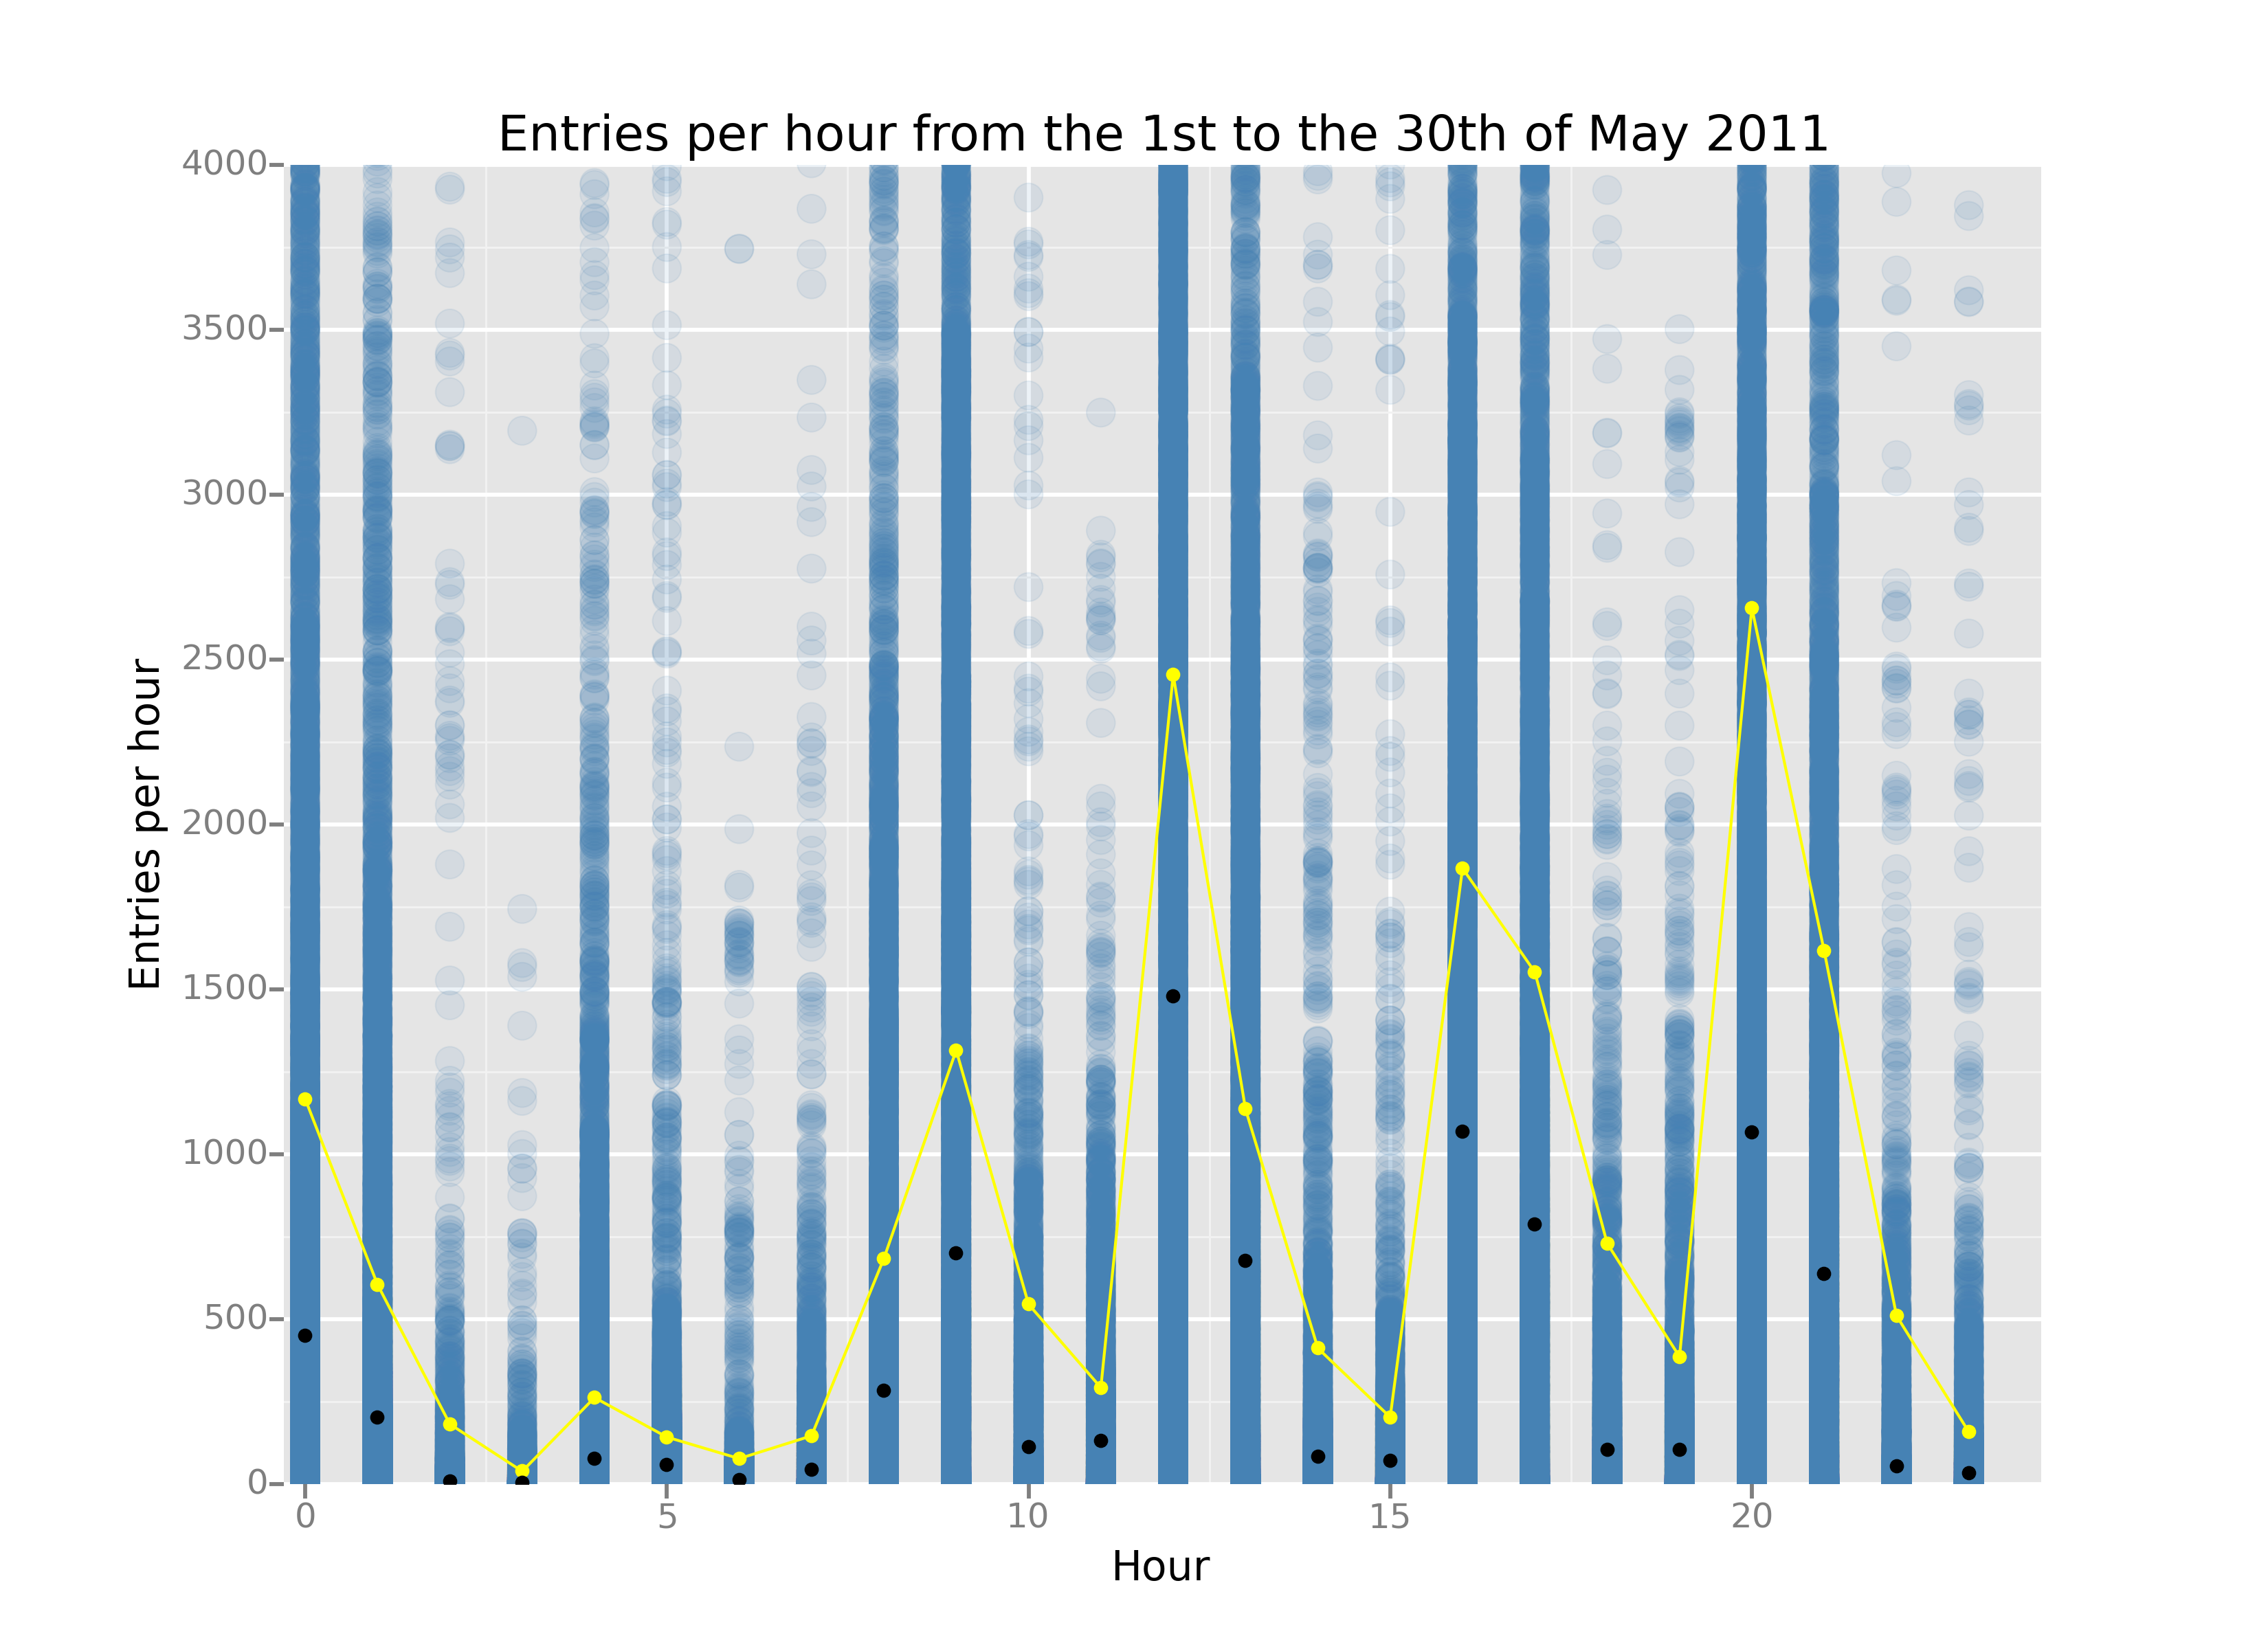
\includegraphics[width=\textwidth]{entries_per_hour.png}
  \caption{Each semi-transparent dot represents a point of data graphed for each
    hour in respect to the number of entries per hour rate.  All outliers
    greater than $4,000$  were left out of the plot in order to provide a more
    meaningful view of the population.  The average and median values are
    represented by the yellow and black dots respectively, and use all values
    including above the $4,000$ level.  Note how even here most of the average
    values are much below $500$ and that there are at least two distinct peaks
  at 12PM and 8PM.}
  \label{fig:bar-graph-ccs-vs-ics-times}
\end{figure}


\begin{problem}
  Visualization II
\end{problem}

I decided to just do a variation on the same theme as the previous
visualization.  This time, however, I've taken the top 6 stations in respect to
the total number of colors needed for representation and plotted their data with
respect to the hours.  What is of note is that it appears many stations are
often times nearly unused for several hours

\newpage

\begin{mdframed}[linecolor=black, topline=true, bottomline=true,
  leftline=false, rightline=false]
\footnotesize
\begin{python1}
from pandas import *
from ggplot import *

def plot_weather_data(turnstile_weather):
    # Get sorted list of stations by the sum of ENTRIESn: 
    by_unit = turnstile_weather.loc[:,['ENTRIESn_hourly' , 'UNIT']]
    by_unit = by_unit.groupby('UNIT').sum()
    by_unit = by_unit.sort_values('ENTRIESn_hourly',ascending = False)

    # Filter stations with at least 1/3 of the largest data point:
    by_unit_cut = by_unit[by_unit > by_unit.iloc[0]/3]
    # PANDAS is nice enough to keep the original df structure so drop NaN
    # values:
    by_unit_cut = by_unit_cut.dropna()

    # reduce total number of stations to 6, 
    # too messy to see much of anything without minimizing this number
    if by_unit_cut.count()[0] > 6: 
        by_unit_cut = by_unit_cut[0:6]

    # Use the generated list to filter out all of the data from the origial
    # data frame:    
    by_unit_data = turnstile_weather.loc[turnstile_weather['UNIT']
    by_unit_data = by_unit_data.isin(by_unit_cut.index.tolist())]

    # Now generate a similar plot as above using a different colors for the 11 
    # stations considered:

    by_unit_data = by_unit_data[['UNIT','ENTRIESn_hourly','Hour']]
    by_unit_data = by_unit_data.sort_values('Hour')
    by_unit_data = by_unit_data.groupby(['UNIT','Hour'], \
        as_index=False).sum()
    
    title = \
    "Entries per hour from the top 6 Stations during May 2011 1st through 30th"
    xlable = "Hour"
    ylable = "Entries per hour"

    plot = ggplot(by_unit_data, + \
        aes(x='Hour', y='ENTRIESn_hourly', color='UNIT')) + \
        geom_point(size=100) + \
        geom_point() + \
        xlab(xlable) + ylab(ylable) + ggtitle(title) + \
        xlim(-.3,24) + ylim(0,400000)

    return plot
\end{python1}
\end{mdframed}

\printbibliography[keyword=Python , title={Python references}]
\printbibliography[keyword=SQL , title={SQL references}]
\printbibliography[keyword=Udacity , title={Udacity references}]
%\printbibliography[keyword=LaTeX , title={{pdf\LaTeX}  references}]
\printbibliography[keyword=statistics , title={Statistics references}]
\printbibliography[keyword=machine.learning, title={Machine Learning references}]
\printbibliography[keyword=ggplot , title={ggplot references}]
\printbibliography[keyword=other , title={other references}]
% 400 billion gallons of water California is roughly 10% of the population
% 20 million
% 100-200 ~ 2-4 bgd 
% ~40 bgd 
\end{document}
